\section{The shape sphere, solved exactly}\label{sec:shape}

\subsection{Coordinates}

Three equal unit masses in the plane, centred and at unit inertia. Jacobi coordinates
$\varrho=(z_1-z_2)/\sqrt2$ and $\varsigma=(z_1+z_2-2z_3)/\sqrt6$ satisfy
$\abs{\varrho}^2+\abs{\varsigma}^2=1$, so the preshape space is the unit sphere $S^3\subset\C^2$;
the diagonal $U(1)$ acts by simultaneous rotation and the shape space is
$S^3/U(1)=\C P^1$, a round sphere of radius $1/2$. Writing
$\varrho=\cos\alpha\,e^{i\varphi_1}$, $\varsigma=\sin\alpha\,e^{i\varphi_2}$ and
$\psi=\varphi_1-\varphi_2$, the quotient metric is
\begin{equation}\label{eq:shapemetric}
   \df s^2=\df\alpha^2+\sin^2\alpha\cos^2\alpha\;\df\psi^2,\qquad 0<\alpha<\tfrac\pi2 .
\end{equation}
With $s=\sin\alpha$ and $c=\cos\alpha$, the squared mutual distances are
\begin{equation}\label{eq:distances}
   x:=d_{12}^2=2c^2,\qquad
   y:=d_{13}^2=\tfrac12+s^2+\sqrt3\,sc\cos\psi,\qquad
   z:=d_{23}^2=\tfrac12+s^2-\sqrt3\,sc\cos\psi,
\end{equation}
so that $x+y+z=3$ on the whole shape sphere. The collinear shapes are $\psi\in\{0,\pi\}$ (the
equator in these coordinates); the two equilateral shapes are $(\alpha,\psi)=(\pi/4,\pm\pi/2)$
(antipodal points at geodesic distance $\pi/2$ from the equator). Three points are
\emph{collisions} ($\alpha\to0$ or $\alpha\to\pi/2$, and the corresponding limits), where the
distance map is not differentiable.

Let $\Phi=(d_{12},d_{13},d_{23})$, let $M$ be its differential in an orthonormal frame, and let
$\sigma_1^2\ge\sigma_2^2$ be the eigenvalues of $M^*M$.

\begin{theorem}[Sum rule for the three-body distance map]\label{thm:shape-sum}
$\sigma_1^2+\sigma_2^2=3$ identically on the regular part of the shape sphere.
\T\ Two independent proofs: (i) Theorem~\ref{thm:perpairs} with unit masses gives
$\norm{\nabla d_a}^2=2-d_a^2$ for each of the three distances, and summing with $x+y+z=3$ gives
$6-3=3$; (ii) direct computation in the frame \eqref{eq:shapemetric}. \V\ Gate
\gate{g01\_shape\_spectrum} (a), $49$ shapes, deviation $2.2\times10^{-9}$.
\end{theorem}

\begin{theorem}[Exact determinant]\label{thm:shape-det}
Let $A$ be the area of the triangle with squared sides $x,y,z$. Then
\begin{equation}\label{eq:det}
   \det M^*M=\frac{12A^2}{xyz}=\frac{9\,s^2c^2\sin^2\psi}{xyz}
   =\frac{3\bigl(2(xy+yz+zx)-x^2-y^2-z^2\bigr)}{4xyz},
\end{equation}
and $\det M^*M\le 9/4$ with equality exactly at the two equilateral shapes; $\det M^*M=0$ exactly
on the collinear locus.
\T\ Proof below. \V\ Gate \gate{g01\_shape\_spectrum} (b),(c),(h): the closed form over $81$
shapes to $1.5\times10^{-9}$, the rank drop on the equator, and the maximum over a grid.
\end{theorem}

\begin{proof}
In the orthonormal coframe $(\df\alpha,sc\,\df\psi)$, the rows of $M$ are
$M_{a1}=\partial_\alpha d_a^2/(2\sqrt a)$ and $M_{a2}=\partial_\psi d_a^2/(2sc\sqrt a)$ for
$a=x,y,z$. Lagrange's identity in two dimensions gives
$\det M^*M=\sum_{a<b}(A_aB_b-A_bB_a)^2/(16s^2c^2ab)$ with $A_a=\partial_\alpha d_a^2$,
$B_a=\partial_\psi d_a^2$. From \eqref{eq:distances}, $A_x=-4sc$, $B_x=0$,
$A_y=2sc-\sqrt3\cos2\alpha\cos\psi$, $B_y=-\sqrt3sc\sin\psi$ and $A_z=2sc+\sqrt3\cos2\alpha\cos\psi$,
$B_z=+\sqrt3sc\sin\psi$, so all three cross products equal $\pm4\sqrt3s^2c^2\sin\psi$ in absolute
value. Hence $\det M^*M=48s^4c^4\sin^2\psi\,(x+y+z)/(16s^2c^2xyz)=9s^2c^2\sin^2\psi/(xyz)$, using
$x+y+z=3$; the Heron form follows from $16A^2=2(xy+yz+zx)-x^2-y^2-z^2$ and
$16A^2=12s^2c^2\sin^2\psi$.
For the bound, write $x=1+u$, $y=1+v$, $z=1+w$ with $u+v+w=0$ and $S=u^2+v^2+w^2$. Then
$16A^2=3-2S$ and $xyz=1-S/2+uvw$, so
\[
   \det M^*M\le\tfrac94 \iff \tfrac{3(3-2S)}{4(1-S/2+uvw)}\le\tfrac94 \iff uvw\ge-\tfrac{S}{6}.
\]
On the circle $u+v+w=0$, $u^2+v^2+w^2=S$, the product $uvw$ is minimised at two equal
variables, giving $uvw\ge-2(S/6)^{3/2}$, and $-2(S/6)^{3/2}\ge-S/6$ exactly when $S\le3/2$,
which is the triangle inequality $16A^2=3-2S\ge0$. Equality forces $S=0$, i.e.\ $x=y=z=1$.
\end{proof}

\begin{theorem}[The cone is linear and isotropic]\label{thm:cone}
Let $\delta$ be the geodesic distance on the shape sphere from an equilateral shape. Then
\begin{equation}\label{eq:cone}
   \sigma_1^2-\sigma_2^2=\sqrt{9-4\det M^*M}=3\,\delta+O(\delta^2),
   \qquad \det M^*M=\tfrac94-\tfrac94\delta^2+O(\delta^3),
\end{equation}
with the same slope $3$ in every direction. On the collinear locus the rank drops to $1$ and the
squared gap is $3$, its maximal value. The determinant has \emph{no} continuous extension to a
collision: at the $23$-collision it tends to $0$ along the collinear meridian and to $2$ along
$\alpha=\pi/6$.
\T/\V\ Gate \gate{g01\_shape\_spectrum} (d): slopes $3.0000$ in four directions with spread
$5\times10^{-5}$; quadratic Hessian of $\det$ equal to $-4.5$; collision limits from
\gate{results/swarm/D8\_m3.md}.
\end{theorem}

\begin{remark}[Two maps, two operators, and one mistake of ours]\label{rem:twomaps}
The statements above are about the \emph{distance} map $\Phi=(d_{12},d_{13},d_{23})$. The
operator-first three-body paper \Cc{} \cite{corpus3b} studies instead the map to the
\emph{squared} distances, $x\mapsto x^{2}$ componentwise, which is a different operator with a
different spectrum, and both are correct. At the equilateral shape of the equal-mass problem:
\begin{center}
\begin{tabular}{@{}lccc@{}}
\toprule
map & $\operatorname{tr}M$ & $\sigma_1^2-\sigma_2^2$ near it & eigen-line holonomy \\
\midrule
distances $\Phi$ (this paper) & $3$ (constant) & $3\delta+O(\delta^2)$ & $-1$ \\
squared distances (the three-body paper) & $6(1+\cos^2\vartheta)$ & $24\,\delta^2+O(\delta^3)$ & $+1$ \\
\bottomrule
\end{tabular}
\end{center}
So the closing is \emph{linear} for the distance map and \emph{quadratic} for the squared-distance
map, and the holonomy is $-1$ for the first and $+1$ for the second. Neither paper is in error.
In the three-body paper's normalisation the squared-distance operator has
$\lambda_{\min}=\cos^2\vartheta$ and $\lambda_{\max}=1$ exactly, with no dependence on the
longitude; we recover $\lambda_{\max}\equiv6$ and $\lambda_{\min}=6\cos^2\vartheta$ for the same
operator before dividing by that constant, which is a check on the identification rather than a
disagreement.

An earlier draft of this paper compared the distance map's numbers against the squared-distance
map's formula and concluded that the quadratic closing was an error. That conclusion was ours and
it was wrong: the two maps are different, and each statement is true of its own. The accurate
statement, which is stronger than either paper alone, is that \emph{taking the square root of the
distances is what creates the cone}: squaring is a smooth reparametrisation that turns a fold into
a simple degeneration and removes the sign change around the loop.
\end{remark}

\begin{theorem}[Holonomy $-1$ for the distance map]\label{thm:shape-holonomy}
For the distance map $\Phi$, the eigen-line of $M^*M$ belonging to $\sigma_1^2$ has holonomy
$-1$ around each equilateral shape; equivalently, with $w=\pm1$ the winding of the two-band
family, $\exp(i\gamma)=(-1)^w$ as in Theorem~\ref{thm:winding}. For the squared-distance map the
same loop returns the eigen-line to itself (holonomy $+1$); see Remark~\ref{rem:twomaps}.
\T\ (Theorem~\ref{thm:winding}(c) applied to the two-band model of the cone, of which
\eqref{eq:cone} is the local form). \V\ Gate \gate{g01\_shape\_spectrum} (e): loop radii
$10^{-2}$ and $3\times10^{-3}$, measured holonomy $-1.000000$ in both; the squared-distance
value $+2\pi$ measured in \gate{notes/07\_TWO\_MAPS.md}.
\end{theorem}

\begin{figure}[t]
\centering
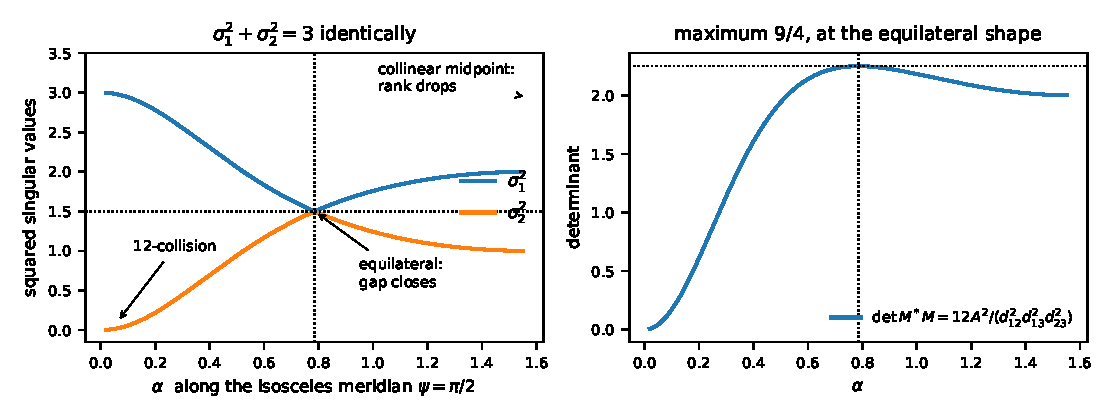
\includegraphics[width=\textwidth]{fig_sheets.pdf}
\caption{Left: the two squared singular values of the shape$\to$distance differential along
the isosceles meridian $\psi=\pi/2$, running from the $12$-collision ($\alpha\to0$) through the
equilateral shape to the collinear midpoint configuration ($\alpha\to\pi/2$). Their sum is $3$ at
every $\alpha$ (Theorem~\ref{thm:shape-sum}); they meet at the equilateral shape, where the gap
closes linearly, and separate toward $(3,0)$, where the rank drops (Theorem~\ref{thm:cone}). Right: the determinant
$12A^2/(d_{12}^2d_{13}^2d_{23}^2)$, maximal and equal to $9/4$ exactly at the equilateral shape
(Theorem~\ref{thm:shape-det}). Both panels are drawn from
\gate{scripts/gates/g01\_shape\_spectrum.py}, not from a separate computation.}
\label{fig:sheets}
\end{figure}

\subsection{Reading the two sheets, and the rigidity that survives}

For equal masses, write $\sigma_\pm^2=\tfrac12\bigl(3\pm\sqrt{9-4\det}\bigr)$. The two sheets
coincide exactly at the equilateral shapes --- the optic points of the birefringent reading ---
and separate on the collinear locus into $(3,0)$. With unequal masses both statements change, and
Theorem~\ref{thm:optic} says how.

\begin{remark}[Rigidity is a choice of variable, not a law to be corrected]\label{rem:rigidity}
For the distance map, $\rho:=\sigma_{\min}^{-2}=2/(3-\sqrt{9-4\det})$ takes the value $2/3$ at the
equilateral shapes and grows like $A^{-2}$ toward the collinear locus. For the squared-distance
map the same definition gives $(\lambda_{\min}/6)^{-2}=\sec^4\vartheta$, since that operator's
$\lambda_{\min}=6\cos^2\vartheta$ (Remark~\ref{rem:twomaps}); this is precisely the three-body
paper's $\rho=\sec^4\vartheta$. The two are not rival values of one quantity: they are
$\sigma_{\min}^{-2}$ for two different operators, and near the collinear locus \emph{both} maps
have $\sigma_2^2\sim\rho_{\mathrm{geom}}^2$ (measured exponent $2.0000$ for each, gate
\gate{g06}, \gate{notes/07\_TWO\_MAPS.md}), so neither exponent is inherited from the
cone-versus-fold distinction. An earlier draft called the fourth power an error inherited from a
mis-stated closing; that was wrong, and the two powers are two definitions.
\end{remark}

\begin{theorem}[The optic points, and what mass breaking does to them]\label{thm:optic}
Let the three masses be arbitrary and let $\sigma_1\ge\sigma_2$ be the singular values of the
distance differential on the shape sphere. Then, for every mass choice we tested, the set of
shapes where $\sigma_1=\sigma_2$ consists of two antipodal points, and at each of them the
degeneracy is a cone. For equal masses the two points are the equilateral shapes and the cone is isotropic
of slope $3$. For unequal masses:
\begin{enumerate}[label=(\roman*)]
\item the two optic points are \emph{displaced} from the equilateral shapes, by a geodesic
distance $=\varepsilon^2/9+O(\varepsilon^3)$ for the family $(1,1,1+\varepsilon)$;
\item the cone at the displaced point is \emph{elliptic}: at $(1,1,2)$ the Hessian of
$\sigma_1^2-\sigma_2^2$ squared has eigenvalues $10.25$ and $13.73$ instead of $(18,18)$;
\item consequently the equilateral shape is \emph{not} an optic point: the gap there is
$3\times$ its distance to the nearest optic point, i.e.\ $\varepsilon^2/3+O(\varepsilon^3)$
for $(1,1,1+\varepsilon)$, and $0.1$ for $(1,1,2)$.
\end{enumerate}
\T/\V\ Gate \gate{g03\_mass\_breaking} (20 assertions), for the mass choices tested: two optic
points in each case, isotropy at equal masses and ellipticity at $(1,1,2)$, displacement exponent $1.995$, displacement
coefficient $0.1096$ against $1/9$, gap-at-equilateral values $0.1$ and $0.196970$ for
$(1,1,2)$ and $(1,2,3)$.
\end{theorem}

\begin{remark}[What mass breaking does, on each map]\label{rem:biaxial}
The three-body paper states that breaking the mass symmetry turns a trivial $+1$ holonomy into
$-1$. On its own operator that is \emph{correct}, and we verify it: for the squared-distance map
the single touching point at equal masses has holonomy $+2\pi$ (sign $+1$), and at masses
$(1,1,1.3)$, $(1,1,2)$ and $(1,2,3)$ it splits into exactly two points, each with holonomy $+1\pi$
(sign $-1$) --- measured at $\alpha$ and $\psi$ listed in \gate{notes/07\_TWO\_MAPS.md}. An
earlier draft of this paper called that prediction wrong; it is not, and the error was ours.
Theorem~\ref{thm:optic} is the corresponding statement for the \emph{distance} map, where the two
touching points are present at equal masses already, are displaced by $\varepsilon^2/9$ and become
an elliptic cone; the two statements describe two operators and do not compete.
\end{remark}
